\documentclass[11pt]{article}

% Change "review" to "final" to generate the final (sometimes called camera-ready) version.
% Change to "preprint" to generate a non-anonymous version with page numbers.
\usepackage[review]{acl}

% Standard package includes
\usepackage{times}
\usepackage{latexsym}

% For proper rendering and hyphenation of words containing Latin characters (including in bib files)
\usepackage[T1]{fontenc}

% This assumes your files are encoded as UTF8
\usepackage[utf8]{inputenc}

% This is not strictly necessary, and may be commented out,
% but it will improve the layout of the manuscript,
% and will typically save some space.
\usepackage{microtype}

% This is also not strictly necessary, and may be commented out.
% However, it will improve the aesthetics of text in
% the typewriter font.
\usepackage{inconsolata}

%Including images in your LaTeX document requires adding
%additional package(s)
\usepackage{graphicx}

% Additional packages
\usepackage{booktabs}
\usepackage{amsfonts}
\usepackage{amsmath}
\usepackage{nicefrac}
\usepackage{algorithm}
\usepackage{algpseudocode}

% \title{Training Language Models to Pass the User Turing Test}
\title{Learning User Simulators with  Turing Rewards}

\author{First Author \\
  Affiliation / Address line 1 \\
  Affiliation / Address line 2 \\
  \texttt{email@domain} \\\And
  Second Author \\
  Affiliation / Address line 1 \\
  Affiliation / Address line 2 \\
  \texttt{email@domain} \\}

\begin{document}
\maketitle

\begin{abstract}
  The abstract paragraph should be indented \nicefrac{1}{2}~inch (3~picas) on both the left- and right-hand margins. Use 10~point type, with a vertical spacing (leading) of 11~points. The word \textbf{Abstract} must be centered, bold, and in point size 12. Two line spaces precede the abstract. The abstract must be limited to one paragraph.
\end{abstract}

\section{Introduction}
The currently dominant use case of LLMs involves having them act as helpful assistants to human users. However, a growing range of applications would benefit  from their playing  the opposite role, i.e.,  not the assistant, but the user.
% Such user simulators could serve as testbeds for conversational agents~\citep{naous2025flipping}, training environments for interactive systems~\citep{abdulhai2025consistently, mehri2025goal}, and proxies for studying human responses at scale~\citep{park2023generative, aher2023simulating, lu2025multiturn}.
Such user simulators could serve as fundamental building blocks for social world models in AI agents \cite{rabinowitz2018machine, collins2024building}, training environments and testbeds for interactive systems~\citep{abdulhai2025consistently, mehri2025goal}, and proxies for studying human responses at scale~\citep{park2023generative, aher2023simulating, lu2025multiturn}.

To simulate a person is to model what makes them \textit{them}. This is fundamentally difficult: users are not interchangeable, and what distinguishes one person from another resists easy categorization. Two people with identical demographics can hold sharply different opinions~\citep{hwang2023aligning, santurkar2023opinions}, and individual preferences cannot be recovered from group-level labels alone~\citep{jiang2024indievalue, kirk2024prism}. Recent work has begun addressing this challenge through purpose-built user language models~\citep{naous2025flipping}, latent user-state alignment~\citep{wu2026humanlm}, log-probability maximization with latent reasoning~\citep{gandhi2026dialogue}, and persona induction from interaction history~\citep{ryan2025synthesizeme}. These approaches share a common assumption: the training signal is derived from matching a specific ground-truth response, whether by scoring similarity against it with an LLM judge or by directly maximizing its log-probability. Such strategies overlook a basic property of human communication, where the same person in the same context could say many different things, all authentically their own. An effective user simulator model should therefore go beyond replicating the ground-truth response, and instead produce responses indistinguishable from what the user {could have said}, i.e., it should pass the Turing Test \citep{turing1950computing}.

% such strategies which encourage models to replicate the ground-truth response is not goal of user simulation, where we are interested in not necessarily  faithful simulator is not to merely reproduce what the user happened to say, but to produce responses indistinguishable from what the user could have said.

% This overlooks a basic property of human communication, where the same person in the same context could say many different things, all authentically their own.

This paper describes a recipe for learning user simulator models based on a \emph{discriminative Turing reward} that asks whether the generated response is distinguishable from the real user's writing, conditioning the model on the user's raw behavioral history together with an induced persona. We validate this recipe through targeted ablations across two dimensions. First, we compare three training signals: a response-similarity reward adapted from HumanLM~\citep{wu2026humanlm}, log-probability maximization with latent chain-of-thought~\citep{gandhi2026dialogue}, and our discriminative Turing reward. The Turing reward consistently outperforms both alternatives. Second, we test how much each component of the user representation contributes by comparing history-only, persona-only, and the combined representation. We find that the combination is critical: history provides raw behavioral evidence while the induced persona supplies a compressed summary of stable traits, and each complements the other.

We evaluate across two settings that differ substantially in structure and register: multi-turn human--LLM dialogue~\citep{kirk2024prism} and Reddit forum discussions~\citep{chang2020convokit}. Our results show that the Turing-trained model not only excels on its own metric but also generalizes to response similarity and state alignment evaluations~\citep{wu2026humanlm}, improving over untrained baselines and alternative training signals on both.

\section{Learning User Simulators}
% \section{Method}

\subsection{Problem Formulation}\label{sec:problem}

We study individual user simulation: given an interaction context and information about a specific person, generate a response that the person could plausibly have produced.

Formally, given triples $(u, x, y)$, $x$ is the immediate interaction context (e.g., a dialogue history or a forum thread), and $u$ is user-specific information about the target individual beyond what appears in $x$. $y$ is one ground-truth response produced by that person.

We observe that $y$ is only a single sample from a broader distribution $p^\star(\cdot \mid x, u)$ of responses the user could authentically produce: the same person in the same context could say many different things, all genuinely their own. Our goal is therefore not to reproduce the specific $y$ in the training data, but to learn a simulator $p_\theta(\hat{y} \mid x, u)$, parameterized by $\theta$, that approximates $p^\star$ such that generated $\hat{y}$ are truly representative of the user utterance's goal, style, and perspective.

The simulator generates a joint sequence $(z, \hat{y}) \sim p_\theta(\cdot \mid x, u)$, where $z$ is a chain-of-thought reasoning trace produced before the response. The trace is masked from reward computation and evaluation; only $\hat{y}$ is scored.

\subsection{User Representation}

We hypothesize that pairing raw behavioral history with an induced persona yields a more faithful user representation than either alone. Concretely, our proposed recipe uses $u = (h, \rho)$: the user's raw behavioral history $h$ (prior utterances or posts not present in $x$) together with an induced persona $\rho$ (a compact natural-language summary of stable traits derived from $h$ by a language model). In our ablation experiments, we also evaluate $u = h$ (history only) and $u = \rho$ (persona only) to isolate the contribution of each component.

\paragraph{History Messages.}
For each user, we reserve a fixed block of $k$ prior interactions, denoted $h$, once at dataset construction and reuse it across every prediction target for that user; the same block is the sole input to persona induction. We require $h$ to be disjoint from the current target context $x$ and ground-truth response $y$, so that the user representation is never contaminated by the example being predicted. The size $k$ is sampled per user from a small range, trading off the strength of the identity prior against the number of remaining targets.

\paragraph{Persona Induction.}
We prompt a language model to summarize stable traits from the user's reserved history block $h$, yielding the persona $\rho$.

The persona is structured along five dimensions: \emph{values} (recurring priorities and themes), \emph{verbal features} (surface-form habits such as punctuation and formatting), \emph{expression style} (tone, formality, directness), \emph{length prior} (typical response length), and \emph{background} (self-disclosed roles, experiences, and domain familiarity). Each dimension is described by one to three concise sentences. Formally, $\rho = f_{\text{LM}}(h)$, where $f_{\text{LM}}$ is a fixed inducer model. Note that $\rho$ depends only on $h$ and never on the current target context $x$ or ground-truth response $y$.

\subsection{Discriminative Turing Reward}\label{sec:training}

We train all models using Group Relative Policy Optimization~\citep[GRPO;][]{shao2024deepseekmath}, sampling $G$ candidate responses per example and computing advantages via within-group normalization.

The Turing reward asks whether a generated response could pass for the real person. An LLM judge is shown the user's behavioral history alongside two responses to the same context: one written by the real user and one generated by the model, assigned to positions A and B at random. The judge rates on a 1--7 scale which response was written by the human, considering consistency with the user's prior writing, stylistic fit, and naturalness. We canonicalize the rating into a score $s^*$ reflecting the judge's confidence that the \emph{candidate} is the real human response:
\begin{equation}
  s^* = \begin{cases} 8 - s & \text{if the candidate is Response A} \\ s & \text{if the candidate is Response B} \end{cases}
\end{equation}
and normalize to obtain the reward $r_{\mathrm{turing}} = (s^* - 1) / 6 \in [0, 1]$, where 0 means the candidate was identified as synthetic with maximum confidence, 0.5 means the judge could not distinguish the two, and 1 means the candidate was mistaken for the real user. Rather than optimizing for content overlap with a specific ground-truth response, this signal trains the model toward the broader quality of being indistinguishable from the target user.

\section{Experimental Setup}

\subsection{Datasets}

We evaluate across two interaction formats that differ in structure, register, and social context.

\paragraph{Multi-turn dialogue (PRISM).}
The PRISM Alignment Dataset~\citep{kirk2024prism} contains 8,011 multi-turn conversations between human participants and LLM assistants, spanning 1,500 participants from 75 countries. Each conversation consists of alternating user and assistant turns, where participants engage with one of 21 LLMs on topics of their choosing, often involving subjective or value-laden questions. We qualify users with at least 6 conversations, yielding 1,288 users. To keep supervised cold-start training disjoint from reinforcement learning, we hold out 10\% of users at random for evaluation (128 users, 880 examples), then split the remaining users into separate GRPO and SFT pools: 696 users for GRPO train/validation and 464 users for SFT. For each user, 2--4 conversations are reserved as behavioral history for constructing the user representation $u$; the rest serve as prediction targets. Because PRISM conversations are linear dialogues, we perform turn-level augmentation: each target conversation produces one training example per user turn, where the current context is all preceding turns and the ground truth is the user's utterance at that turn.

\paragraph{Online forum discussion (ConvoKit).}
The ConvoKit subreddit corpus~\citep{chang2020convokit} contains threaded Reddit discussions across a range of communities. We select 14 subreddits and qualify users who participate in at least 8 threads, yielding 1,282 users. To keep supervised cold-start training disjoint from reinforcement learning, we partition non-held-out users into separate SFT and GRPO pools: 472 users for SFT and 707 users for GRPO train/validation. We hold out \texttt{r/tifu} and \texttt{r/worldnews} for evaluation, yielding 102 test users and 267 test examples, with no user overlap with either training pool. For each user, 2--6 threads are reserved as behavioral history; the remaining threads serve as targets. Because Reddit threads are branching and expanding every user reply within a thread would create highly correlated examples, we use a single prediction target per thread: the user's last comment, with their earlier comments in the same thread retained as context.

\subsection{Evaluation}

We evaluate generated responses along three complementary dimensions, each operationalized via an LLM judge.

\paragraph{Turing distinguishability.}
A judge is presented with the user's behavioral history, the interaction context, and two responses: the ground-truth human response and a model-generated candidate, with position randomized. The judge rates which response was written by the real user on a 1--7 scale. To control for position bias, we evaluate each pair in both orderings and average the canonicalized scores. Higher scores indicate the generated response was harder to distinguish from the real one. This metric captures aspects of user fidelity that content-level metrics may miss, such as stylistic consistency and appropriate response length.

\paragraph{Response similarity.}
An LLM judge scores how well a generated response captures the overall content of the ground-truth human response, considering coverage of key points and penalizing extraneous or contradictory material. This yields a single score in $[0, 1]$ measuring whether the model said roughly what the real user said.

\paragraph{State alignment.}
Following \citet{wu2026humanlm}, we separately evaluate alignment along six psychologically grounded dimensions: \emph{stance} (agreement toward an explicit target), \emph{emotion} (affect and intensity toward a target), \emph{belief} (foundational assumptions about people or the world), \emph{value} (what the user treats as important), \emph{goal} (communicative intent of the response), and \emph{communication} (tone and message structure). For each dimension, the judge extracts key aspects from the ground-truth response and scores how well the generated response reflects them. We report both per-dimension scores and the mean across all dimensions.

\subsection{Baselines and Ablations}

Our experiments are organized as follows.

\paragraph{Training signal comparison.}
We fix the user representation to $u = (h, \rho)$ and compare four training conditions: (1)~GRPO with Turing reward (proposed), (2)~GRPO with response similarity reward~\citep{wu2026humanlm}, (3)~GRPO with log-probability and latent thinking~\citep{gandhi2026dialogue}, and (4)~supervised fine-tuning (SFT). We also report the performance of the untrained base model (Qwen3-8B) as a zero-shot reference.

\paragraph{User representation ablation.}
We fix the training signal to the Turing reward and compare three input conditions: $u = h$ (history only), $u = \rho$ (persona only), and $u = (h, \rho)$ (both). This isolates the contribution of each component.

\section{Turing Eval Results}

\begin{figure*}[t]
\centering
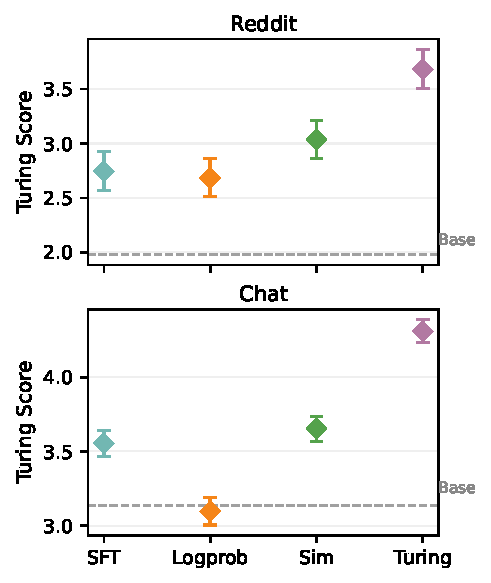
\includegraphics[width=.95\textwidth]{figures/sonnet46_turing_scores.pdf}
\caption{Turing judge scores.}
\label{fig:sonnet46_turing_scores}
\end{figure*}

\begin{figure*}[t]
\centering
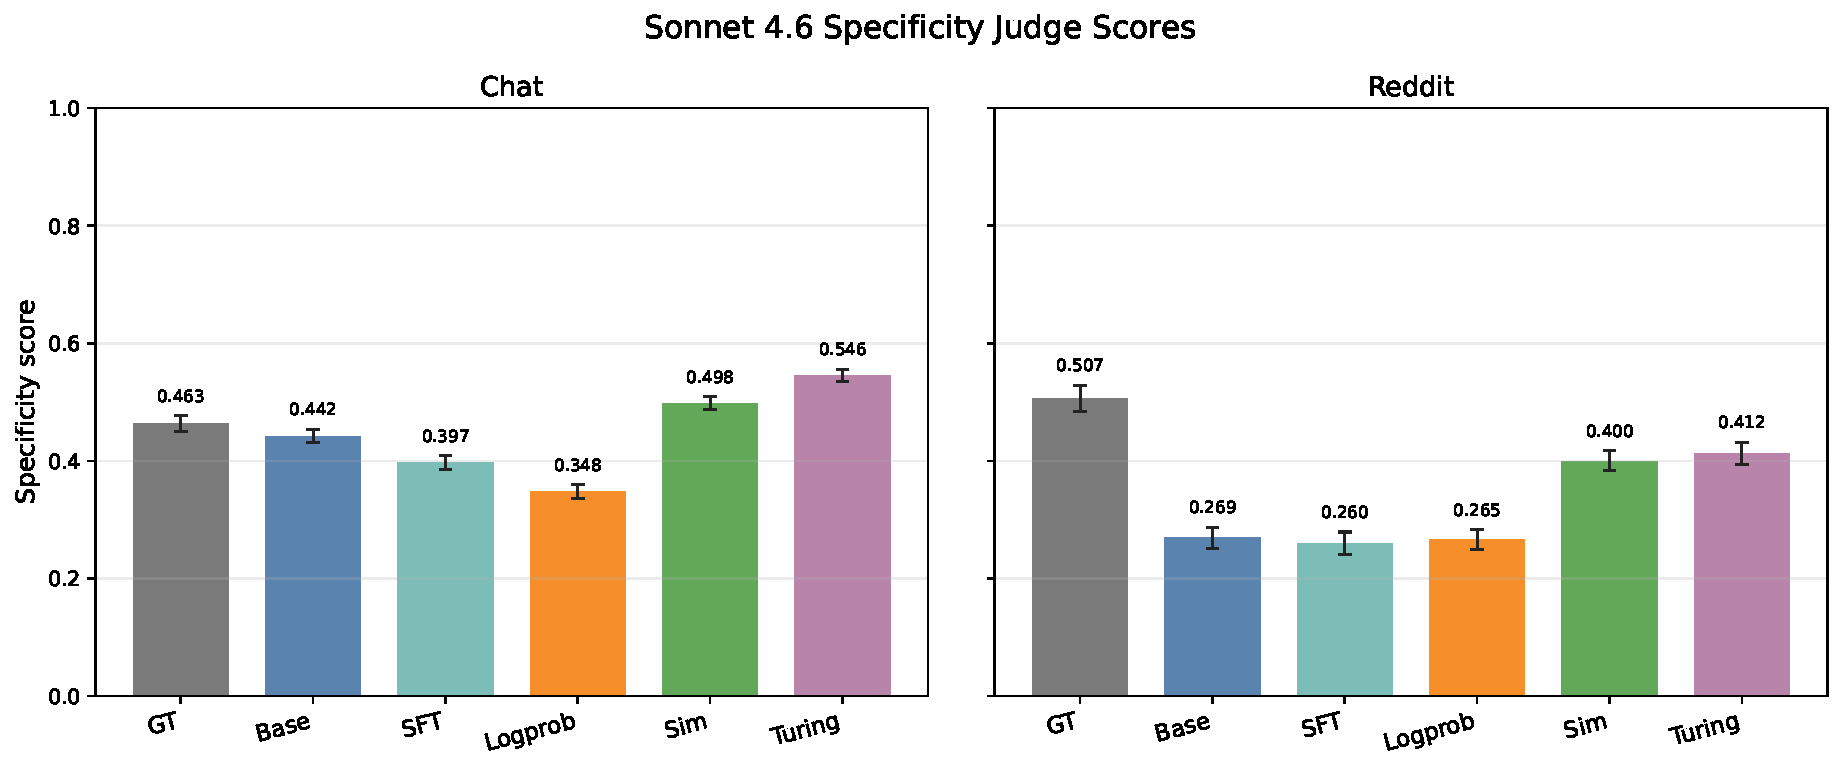
\includegraphics[width=.95\textwidth]{figures/sonnet46_specificity_scores.pdf}
\caption{Specificity judge scores.}
\label{fig:sonnet46_specificity_scores}
\end{figure*}

\subsection{Chat}
on heldout subjects

untrained / sft / grpo-logprob / grpo-turing 
\subsection{Reddit}
\section{Latent State Eval Results}
\subsection{Chat}
\subsection{Reddit}
\section{Human Evaluation and Systems Level Comparison}

\section{Analysis: Input Space Ablations}

\section{Discussion}

\section{Related Work}

\paragraph{LLM-based user simulation.}
LLMs have been used to evaluate dialogue systems~\citep{davidson2023user, sekulic2024simulating}, train conversational agents via self-play~\citep{shah2018bootstrapping, abdulhai2025consistently}, and replicate human subject studies~\citep{aher2023simulating, park2023generative}. \citet{naous2025flipping} show that assistant-tuned LLMs are structurally misaligned with the user role, while \citet{mehri2025goal} address goal drift in task-oriented simulation through explicit state tracking. These works establish that user simulation benefits from purpose-built training but model generic users rather than specific individuals.

\paragraph{Representing individual users.}
Persona-conditioned generation was introduced by \citet{zhang2018personalizing} and extended with pretrained models by \citet{wolf2019transfertransfo}. Subsequent work enriches user representations: \citet{hwang2023aligning} show that retrieving relevant past opinions outperforms demographic prompting; \citet{ryan2025synthesizeme} induce synthetic personas from behavioral traces for personalized reward modeling; and \citet{jiang2024indievalue} demonstrate that individual values cannot be approximated by group-level categories. We combine raw history with an induced persona, providing both behavioral evidence and a compressed trait summary.

\paragraph{Training objectives for human simulation.}
Beyond standard supervised fine-tuning~\citep{wolf2019transfertransfo}, \citet{wu2026humanlm} optimize for similarity along psychologically grounded dimensions such as stance and emotion, \citet{abdulhai2025consistently} use LLM-judged consistency scores as PPO rewards, and \citet{gandhi2026dialogue} show that log-probability maximization with latent chain-of-thought outperforms judge-based rewards in generic dialogue prediction. Our discriminative Turing reward takes a different approach: rather than matching content or maximizing likelihood, it trains the model to be indistinguishable from the real user. We show this signal generalizes across evaluation metrics and interaction formats.

\section*{Limitations}

\section*{Acknowledgments}

\bibliography{custom}

\appendix

\section{Technical Appendices and Supplementary Material}

\subsection{Generation Prompts}

\subsection{Judge Prompts}

\subsection{Dataset Preprocessing and Statistics}

Each training example is a tuple $(u, x, y)$ where the user representation $u = (h, \rho)$ is fixed per user and disjoint from both the current context $x$ and the ground-truth response $y$. The behavioral history $h$ is selected once per user from a deterministic seed; the persona $\rho$ is induced from $h$ alone. This separation guarantees that neither $h$ nor $\rho$ leaks information about the target.

\paragraph{PRISM.}
We retain PRISM participants with at least six conversations, yielding 1,288 qualified users. We randomly hold out 10\% of qualified users with a fixed seed, giving 128 held-out test users and 880 test examples. The remaining 1,160 users are split with the same seed into disjoint GRPO and SFT pools using a 60/40 user ratio: 696 users for GRPO and 464 users for SFT. Per user, 2--4 conversations are reserved as $h$; the rest serve as targets. Because PRISM dialogues are linear, each user turn in a target conversation is one example: $x$ is all preceding turns and $y$ is the user's utterance at that turn. GRPO train and validation examples are split within each GRPO user using a deterministic tail-split policy: for a user with $n$ target rows, $\lfloor 0.1n \rfloor$ rows, with a minimum of one when $n>1$, are assigned to validation. Before applying this tail split, target rows are sorted by conversation id and target turn index, so validation rows come from later target turns and training does not use a later target from the same conversation than validation.

\paragraph{ConvoKit.}
We reconstruct Reddit threads from comment identifiers and parent pointers. Deleted, removed, and non-user comments cannot serve as targets or enter $h$, but non-root unusable comments may be kept as structural anchors so that descendant replies stay connected to the ancestor chain. We reserve \texttt{r/tifu} and \texttt{r/worldnews} as held-out test subreddits and remove their users from both SFT and GRPO training. The remaining users are split deterministically into disjoint SFT and GRPO pools using a 40/60 ratio. GRPO train and validation examples are then split within each GRPO user using the same deterministic tail-split policy as the preprocessing pipeline: for a user with $n$ target rows, $\lfloor 0.3n \rfloor$ rows, with a minimum of one when $n>1$, are assigned to validation and the earlier rows to training. This gives every GRPO training user at least one validation row; users with only one eligible row are dropped from GRPO train/validation. Per user, 2--6 threads are reserved as $h$. Each target thread yields one example: $y$ is the user's final comment and $x$ is the original post plus the ancestor reply chain leading to it, avoiding highly correlated examples from the same thread.

\begin{quote}
\small
\textbf{SFT/GRPO pool:} AmItheAsshole, AskMen, AskWomen, business, changemyview, Economics, Frugal, MaliciousCompliance, news, relationship\_advice, relationships, TrueReddit \\
\textbf{Held-out test:} tifu, worldnews
\end{quote}

\paragraph{Persona induction.}
We prompt GPT-5.4-nano (temperature 0.2, max 2{,}048 tokens) to summarize each user's history block $h$ into a fixed persona $\rho$ with five fields: values, verbal features, expression style, length prior, and background. The same $\rho$ is reused for every example belonging to that user. Figure~\ref{fig:persona_induction} shows the induction prompt.

\begin{figure*}[t]
\centering
\small
\hrule\vspace{4pt}
\begin{algorithmic}[1]
\Statex \textbf{System message}
\State \texttt{You write compressed first-person persona notes as if the target user}
\Statex \texttt{\quad wrote them about their own habits.}
\State \texttt{Sound like the user, not like an analyst, therapist, teacher, or policy brief.}
\State \texttt{Output only the requested strict JSON object and nothing else.}
\Statex \hrulefill
\Statex \textbf{User message}
\State \texttt{<target\_speaker>[HUMAN]</target\_speaker>}
\State \texttt{<selected\_history>} \textit{(reserved history block $h$, with [HUMAN]/[OTHER] speaker labels}
\Statex \textit{\quad and bold-delimited target-user responses)} \texttt{</selected\_history>}
\State
\State \texttt{<task>}
\State \texttt{Write a compact persona for [HUMAN] in [HUMAN]'s own voice.}
\State
\State \texttt{Rules:}
\State \texttt{- Write each field in first person, as if [HUMAN] is}
\Statex \texttt{\quad describing their own habits.}
\State \texttt{- Keep it casual and compressed, not polished or formal.}
\State \texttt{- Use only [HUMAN]'s own messages as evidence.}
\State \texttt{- Capture only stable traits that are useful for predicting}
\Statex \texttt{\quad future messages across contexts.}
\State \texttt{- Prefer concrete wording habits over abstract summaries.}
\State \texttt{- Do not sound like an analyst describing a person from the outside.}
\State \texttt{- Do not use therapist/assistant/policy-brief language.}
\State \texttt{- Avoid abstract labels such as fairness, accountability, autonomy,}
\Statex \texttt{\quad respect, boundaries, power dynamics, empathy, nuance, skepticism,}
\Statex \texttt{\quad advocacy, procedural correctness, or similar summary words}
\Statex \texttt{\quad unless those exact words are frequent in the history.}
\State \texttt{- Do not infer demographics or sensitive attributes.}
\State \texttt{- Do not infer motives, worldview, morals, personality traits,}
\Statex \texttt{\quad or values unless they are explicitly and repeatedly stated.}
\State \texttt{- Do not include one-off topical stances, transient emotions,}
\Statex \texttt{\quad or local interaction goals.}
\State \texttt{- If evidence is weak, write `unknown`.}
\State \texttt{- Keep each field concise.}
\State \texttt{- Write each field as short fragments or very short sentences,}
\Statex \texttt{\quad not polished mini-paragraphs.}
\State \texttt{- Do not quote or reproduce complete sentences from the}
\Statex \texttt{\quad selected history.}
\State \texttt{- Do not quote or reuse exact words or phrases from the selected}
\Statex \texttt{\quad history, including verdict labels, slang, catchphrases, or short}
\Statex \texttt{\quad text fragments.}
\State \texttt{- Do not include literal examples from [HUMAN]'s messages, even}
\Statex \texttt{\quad single-word examples.}
\State \texttt{- Describe lexical habits generically rather than by repeating}
\Statex \texttt{\quad exact tokens.}
\State \texttt{- Non-text segments such as punctuation styles may be described,}
\Statex \texttt{\quad but do not quote surrounding text.}
\State \texttt{- Do not include parenthetical example lists, `e.g.`}
\Statex \texttt{\quad scaffolding, or full sample sentences from [HUMAN]'s messages.}
\State
\State \texttt{Field descriptions:}
\State \texttt{- values: only concrete recurring preferences, irritations,}
\Statex \texttt{\quad or things I keep siding with; avoid abstract moral language}
\Statex \texttt{\quad unless it is explicit in the history}
\State \texttt{- verbal\_features: my observable surface-form habits only,}
\Statex \texttt{\quad such as how I use interjections, punctuation, grammar}
\Statex \texttt{\quad looseness, discourse markers, formatting quirks, or short}
\Statex \texttt{\quad repeated lexical patterns. Do not include exact verdict}
\Statex \texttt{\quad labels or quoted wording from the history.}
\State \texttt{- expression\_style: how I usually come across at the sentence}
\Statex \texttt{\quad level; keep this concrete and plain, not psychological,}
\Statex \texttt{\quad evaluative, or therapist-like}
\State \texttt{- length\_prior: my usual reply length in plain language,}
\Statex \texttt{\quad mainly sentence count and rough brevity}
\State \texttt{- background: concrete background cues not already captured}
\Statex \texttt{\quad above, especially repeated personal experiences,}
\Statex \texttt{\quad self-disclosed roles, responsibilities, constraints,}
\Statex \texttt{\quad routines, domain familiarity, sources of information,}
\Statex \texttt{\quad or recurring points of reference that likely shape}
\Statex \texttt{\quad future responses; do not restate general values, tone,}
\Statex \texttt{\quad or reasoning style; use `unknown` if nothing strong}
\Statex \texttt{\quad remains}
\State
\State \texttt{Output only this JSON object shape:}
\State \texttt{\{"values": "...", "verbal\_features": "...", "expression\_style": "...",}
\Statex \texttt{\quad "length\_prior": "...", "background": "..."\}}
\State \texttt{</task>}
\Statex \hrulefill
\Statex \textbf{Model output}
\State \texttt{\{"values": "...", "verbal\_features": "...", "expression\_style": "...",}
\Statex \texttt{\quad "length\_prior": "...", "background": "..."\}}
\end{algorithmic}
\vspace{2pt}\hrule
\caption{Persona induction prompt. The inducer receives the user's reserved history $h$ formatted with speaker labels and bold-delimited target-user responses, and outputs a structured JSON persona $\rho$.}
\label{fig:persona_induction}
\end{figure*}

\paragraph{OOD evaluation sets.}
Two small out-of-distribution sets are reserved for evaluation only: Chatbot Arena (50 examples, 23 users, drawn from 94 candidates) and Humanual Opinion (50 examples, 17 users, drawn from 135 candidates). Selection covers every available user first, then fills remaining slots by deterministic round-robin.

\begin{table*}[t]
\centering
\small
\begin{tabular}{lrrrr}
\toprule
 & PRISM & ConvoKit & Chatbot Arena (OOD) & Humanual Op. (OOD) \\
\midrule
Users & 1,288 & 1,282 & 23 & 17 \\
History & 2--4 conv. & 2--6 threads & 2--4 conv. & 2--6 conv. \\
SFT train & 3,272 & 4,264 & --- & --- \\
GRPO train & 4,174 & 4,737 & --- & --- \\
GRPO val & 705 & 1,661 & --- & --- \\
Test & 880 & 267 & 50 & 50 \\
\bottomrule
\end{tabular}
\caption{Dataset statistics after preprocessing. History counts are sampled per user. PRISM and ConvoKit use disjoint SFT, GRPO, and held-out test users; the held-out ConvoKit test set comes from \texttt{r/tifu} and \texttt{r/worldnews}. OOD sets are evaluation-only.}
\label{tab:preprocessing_stats}
\end{table*}

\paragraph{Prompt format.}
Each example is rendered as a two-message chat sequence: a system message containing the simulation instruction, the task description, and (when applicable) the induced persona $\rho$ (Figure~\ref{fig:system_prompt}); and a user message containing the behavioral history $h$ followed by the current context $x$. The model generates a chain-of-thought trace $z$ enclosed in \texttt{<reasoning>} tags, then the response $\hat{y}$ prefixed by \texttt{[HUMAN]:}. Figures~\ref{fig:prism_format} and~\ref{fig:convokit_format} show the user message layout for each dataset.

\begin{figure*}[t]
\centering
\small
\hrule\vspace{4pt}
\begin{algorithmic}[1]
\Statex \textbf{System message (shared across all datasets)}
\State \texttt{You are simulating a human labeled by [HUMAN]. Your job is to predict what [HUMAN] says as if you are that person.}
\State
\State \texttt{[PERSONA]}
\State \texttt{<persona>}
\State \quad \texttt{<values>}...\texttt{</values>}
\State \quad \texttt{<verbal\_features>}...\texttt{</verbal\_features>}
\State \quad \texttt{<expression\_style>}...\texttt{</expression\_style>}
\State \quad \texttt{<length\_prior>}...\texttt{</length\_prior>}
\State \quad \texttt{<background>}...\texttt{</background>}
\State \texttt{</persona>}
\State
\State \texttt{[TASK]}
\State \texttt{Your task is to predict [HUMAN]'s next message, matching [HUMAN]'s writing intentions, style, vocabulary, and tone.}
\State \texttt{Use all provided information about [HUMAN] and the current context to predict the next message.}
\State \texttt{Target your message to [OTHER] or [OTHER - OP], not to people who are described in the context but are not participants}
\State \texttt{in the thread or conversation. Do not answer as an assistant, analyst, or narrator.}
\State
\State \texttt{Before outputting the final answer, briefly reason about what [HUMAN] would say and think step by step.}
\State \texttt{The generated response should naturally follow from your reasoning.}
\State \texttt{Format your output exactly like this:}
\State \texttt{<reasoning>...</reasoning>}
\State \texttt{[HUMAN]: your response}
\State \texttt{Write any reasoning before `[HUMAN]:` enclosed by the reasoning tags, and write only the final response after `[HUMAN]:`.}
\State \texttt{Do not include reasoning after `[HUMAN]:`.}
\end{algorithmic}
\vspace{2pt}\hrule
\caption{System message shared across all prompt configurations. The \texttt{[PERSONA]} block is included only in persona-conditioned settings; the \texttt{[TASK]} block specifies the prediction objective and output format.}
\label{fig:system_prompt}
\end{figure*}

\begin{figure*}[t]
\centering
\small
\hrule\vspace{4pt}
\begin{algorithmic}[1]
\Statex \textbf{User message (PRISM)}
\State \texttt{[USER HISTORY]}
\State \texttt{Below are previous conversations involving [HUMAN]. Use them to infer [HUMAN]'s style, values, preferences, and likely responses.}
\State
\State \texttt{<Conversation 1>}
\State \texttt{[MESSAGES]}
\State \texttt{[HUMAN]:} \textit{user turn}
\State \texttt{[OTHER]:} \textit{assistant turn}
\State \texttt{[HUMAN]:} \textit{user turn}
\State \texttt{[OTHER]:} \textit{assistant turn}
\State \texttt{</Conversation 1>}
\State
\State \texttt{[CURRENT CONTEXT]}
\State \texttt{[MESSAGES SO FAR]}
\State \texttt{[HUMAN]:} \textit{turn 0}
\State \texttt{[OTHER]:} \textit{turn 0}
\State \texttt{[HUMAN]:} \textit{turn 1}
\State \texttt{[OTHER]:} \textit{turn 1}
\Statex \hrulefill
\Statex \textbf{Model output}
\State \texttt{<reasoning>}...\texttt{</reasoning>}
\State \texttt{[HUMAN]:} $\hat{y}$
\end{algorithmic}
\vspace{2pt}\hrule
\caption{User message layout for PRISM (multi-turn dialogue). History conversations are wrapped in numbered \texttt{<Conversation>} tags; the current context lists turns up to the prediction point.}
\label{fig:prism_format}
\end{figure*}

\begin{figure*}[t]
\centering
\small
\hrule\vspace{4pt}
\begin{algorithmic}[1]
\Statex \textbf{User message (ConvoKit)}
\State \texttt{[USER HISTORY]}
\State \texttt{Below are [HUMAN]'s previous messages.}
\State
\State \texttt{<Post 1>}
\State \texttt{[OTHER - OP]}
\State \textit{original post text}
\State
\State \texttt{[OTHER]:} \textit{reply}
\State \texttt{[HUMAN]:} \textit{reply}
\State \texttt{[OTHER]:} \textit{reply}
\State \texttt{</Post 1>}
\State
\State \texttt{[CURRENT CONTEXT]}
\State \texttt{[OTHER - OP]}
\State \textit{original post text}
\State
\State \texttt{[OTHER]:} \textit{ancestor reply}
\State \texttt{[HUMAN]:} \textit{earlier comment}
\State \texttt{[OTHER]:} \textit{ancestor reply}
\State \texttt{[HUMAN]:}
\Statex \hrulefill
\Statex \textbf{Model output}
\State \texttt{<reasoning>}...\texttt{</reasoning>}
\State \texttt{[HUMAN]:} $\hat{y}$
\end{algorithmic}
\vspace{2pt}\hrule
\caption{Prompt layout for ConvoKit (Reddit forum). History threads are wrapped in numbered \texttt{<Post>} tags; the original poster is marked \texttt{[OTHER - OP]}. The current context shows the OP and ancestor reply chain up to the prediction point.}
\label{fig:convokit_format}
\end{figure*}

\subsection{}
\end{document}
